\chapter{Introduction}\label{ch:introduction}
\section{Space Vector Theory} \label{sec:0_sv} 
Due to benefits regarding the mathematical modeling of electrical three-phase system, space vectors are commonly used. The idea behind this, is to describe real-valued three-phase quantities as one complex-valued quantity. By doing so, a change of reference frames is easily achieved (as shown in Section \ref{sec:0_refframes})  and  an intuitive description of the magnitude and phase angle of a three-phase system is provided. \\
For a balanced sinusoidal three-phase current system, the phase currents can be expressed as 
\begin{equation*}
	\begin{split}
		i_a(t) &= I\cos\omega t,\\
		i_b(t) &= I\cos\left(\omega t-\frac{2\pi}{3}\right),\\
		i_c(t) &= I\cos\left(\omega t+\frac{2\pi}{3}\right)
	\end{split}
	\label{equ:0_current_sequence}
\end{equation*}
Those sinusoidal waves with constant angular frequency can be expressed as complex quantities $ \hat{I},\; \hat{I} e^{\J 2\pi/3},\; \hat{I} e^{-\J 2\pi/3}$, with fixed angle of $120^\circ$ relative to each other, as depicted in Figure \ref{fig:0_sv}.
\begin{figure}
	\centering
	\begin{center}
	\begin{tikzpicture}
		\draw[->] (-2.4,0) -- (2.5,0);
		\draw[->] (1.2,-2.1) -- (-1.24,2.1) node[above left=0pt, at end] {$b$};
		\draw[<-] (-1.2,-2.1) -- (1.24,2.1) node[at start, below right] {$c$};
		
		
		\draw[very thick,->] (0,0) -- (1.56,0) node[midway,above] {$\hat{I}_a$};
		\draw[very thick,->] (0,0) -- (-0.78,1.36) node[midway,left] {$\hat{I}_b$};
		\draw[very thick,->] (0,0) -- (-0.78,-1.36) node[midway,left] {$\hat{I}_c$};
		
		\fill (0,0) circle (1.6pt);
	  \draw[->, dashed] (0,-0.2) -- (0,2.89);
	  \draw[->, dashed] (-0.19,0) -- (3.12,0);
	  \node at (3.09,-0.26) {$\alpha$};
	
	  \node at (-0.37,2.83) {$\beta$};

  \node at (2.42,-0.27) {$a$};
\end{tikzpicture}
\end{center}
	\caption{Three phase system definition with complex quantities}
	\label{fig:0_sv}
\end{figure}
The instantaneous phase quantities can be represented by the complex space vector
\[
\underline{i}_{S} = \frac{2}{3} \left( {I} + {I} e^{\J 2\pi/3} + {I} e^{-\J 2\pi/3}  \right).
\]
The scaling factor $2/3$ is chosen such that the magnitude of the space vector corresponds to the amplitude of the balanced three-phase quantity. In general, the use of a complex space vector does not require the three-phase quantities to be sinusoidal or to have a constant frequency. Defining $i_\alpha = \RE\{\underline{i}_{S}\}$ and $i_\beta = \IM\{\underline{i}_{S}\}$, the commonly known Clarke transform for balanced systems, as in three phase system without connection of the neutral star point, can be derived. \\
Even though this transformation seems like a projection, no information is lost when the zero sequence condition $i_a + i_b + i_c = 0$ is considered.

\begin{equation}
	\begin{bmatrix}
		i_\alpha \\
		i_\beta
	\end{bmatrix}
	=
	\underbrace{
		\frac{2}{3}
		\begin{bmatrix}
			1 & -\frac{1}{2} & -\frac{1}{2} \\
			0 & \frac{\sqrt{3}}{2} & -\frac{\sqrt{3}}{2}
	\end{bmatrix}}_{\clarke}
	\begin{bmatrix}
		i_a \\
		i_b \\
		i_c
	\end{bmatrix}.
	\label{equ:0_clarke}
\end{equation}
The real-valued vector $\bm{i}_S^S = [i_\alpha \;i_\beta]^\T$ corresponds to the complex space vector $\underline{i}_S^S = i_\alpha + \J i_\beta$. For modeling purposes, the space vector representation simplifies coordinate system transformations, while the real vector representation is used for control purposes to ensure a real-valued state vector.\\
Although $\clarke$ is not a square matrix, the inverse transform can be defined via the Moore-Penrose pseudo-inverse $\iclarke  = \clarke^{\dagger}$.\\
The Clarke transform can be thought of as a convenient mathematical description for the three phase quantities by using a space vector. As mentioned, this eases the transformation between coordinate systems. This will be shown in the following section.

\section{Reference Frames} \label{sec:0_refframes}
Two reference frames for the stator current and voltage space vector are of interest. The first one is the stationary reference frame (\acrshort{srf}). In this frame of reference the space vector is a direct representation of the quantities, which can be directly measured at the terminals of the machine. Therefore, the constraints, due to the generation of the stator voltage is stationary in this frame of reference. Quantities described in this reference frame are indicated with a superscript $^S$.\\
The permanent magnet flux linkage is fixed relative to the rotor, as is the saliency, which refers to the two inductances $L_d$ and $L_q$. Due to this configuration, it is beneficial to describe the electric and magnetic stator quantities in a rotor fixed reference frame. This frame will be called the rotating reference frame (\acrshort{rrf}). By doing so, the real or direct component of this vector $\RE\{\underline{i}_S^R\} = i_d$ is oriented in the same axis as the flux linkage of the permanent magnets $\underline{\psi}_{PM}$. This leads to positive $i_d$ strengthening the permanent magnet flux linkage, negative $i_d$ weakening it. For non-salient machines $L_d = L_q$, the imaginary or quadrature component $\IM\{\underline{i}_S^R\} = i_q$ directly influences the electric torque. To describe the torque of salient-pole machines, the influence of $i_d$ due to reluctance torque according to the full Torque Relation \eqref{equ:1_pmsm_torque} has to be considered as well.\\
Therefore, $i_d$ is the flux-producing component of the stator current. To ensure minimum stator current for maximum torque, $|i_d$| is kept as low as possible (at base speed, its reference is set to zero and for field-weakening operation $i_d<0$) and $i_q$ is used primarily to influences the electric torque. Space vectors in the rotating frame of reference are marked with a superscript $^R$. 


\subsection{Coordinate Frame Transformation} \label{sec:0_coordtrans}
As mentioned in the previous section, a transformation rule is needed, to translate quantities from the \acrshort{srf} to the \acrshort{rrf} and vice versa.\\
To describe this transformation an arbitrary space vector $\underline{z}$ is considered. In the stationary reference frame, the vector can be expressed as

\begin{equation*}
	\underline{z}^{S}
	=
	z_\alpha + \J z_\beta
	=
	\lvert z\rvert e^{\J\epsilon},
	%	\label{equ:0_sv_srf}
\end{equation*}

where $\epsilon$ denotes the angle of the space vector relative to the $\alpha$-axis. Therefore, its components are given by

\begin{equation*}
	z_\alpha = \RE\{\underline{z}^{S}\}
	= \lvert z\rvert\cos\epsilon,\quad
	z_\beta = \IM\{\underline{z}^{S}\}
	= \lvert z\rvert\sin\epsilon.
	%	\label{equ:0_sv_srf_components}
\end{equation*}

The same space vector can be expressed in the rotating reference frame as

\begin{equation*}
	\underline{z}^{R}
	=
	z_d + \J z_q
	=
	\lvert z\rvert e^{\J\kappa},
	\label{equ:0_sv_rrf}
\end{equation*}

\begin{figure}[h]
	\centering
	
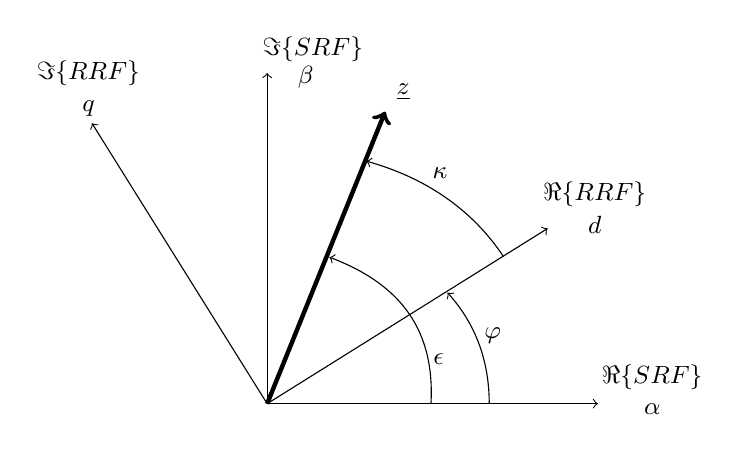
\begin{tikzpicture}[
    axis/.style={->, thick},
    vector/.style={->, very thick},
    angle/.style={->, thick},
    every node/.style={font=\small}
]


\def\R{4.2}        % length of reference axes
\def\angRRF{32}    % phi: RRF rotation relative to SRF
\def\angZ{68}      % epsilon: z angle relative to alpha axis
\def\Vz{4.0}       % magnitude of z


\coordinate (O) at (0,0);

\coordinate (A) at (\R,0);
\coordinate (B) at (0,\R);

\draw[axis, thin] (O) -- (A)
;

\draw[axis, thin] (O) -- (B)
;
\coordinate (D) at ({\R*cos(\angRRF)},{\R*sin(\angRRF)});
\coordinate (Q) at ({\R*cos(\angRRF+90)},{\R*sin(\angRRF+90)});

\draw[axis, thin] (O) -- (D)
;

\draw[axis, thin] (O) -- (Q)
;


\coordinate (Z) at ({\Vz*cos(\angZ)},{\Vz*sin(\angZ)});

\draw[vector, ultra thick, ->] (O) -- (Z)
    node[at end, above right] {$\underline{z}$};


\coordinate (Zd) at
    ({\Vz*cos(\angZ)*cos(\angRRF) +
      \Vz*sin(\angZ)*sin(\angRRF)},
     {(\Vz*cos(\angZ)*cos(\angRRF) +
      \Vz*sin(\angZ)*sin(\angRRF))*sin(\angRRF)});

\node at (0.58,4.5) {$\Im\{SRF\}$};

\node[align=center] at (2.23,0.57) {
    $\epsilon$
};
\node[align=center] at (2.92,0.87) {
    $\varphi$
};
\node[align=center] at (2.25,2.93) {
    $\kappa$
};


  \node at (-2.27,4.19) {$\Im\{RRF\}$};

  \node at (4.89,0.34) {$\Re\{SRF\}$};

  \node at (4.16,2.66) {$\Re\{RRF\}$};
  \draw[->] (2.08,0) .. controls (2.13,0.91) and (1.72,1.51) .. (0.79,1.86);

  \draw[->] (2.82,0) .. controls (2.82,0.54) and (2.65,1.01) .. (2.29,1.41);
  \draw[->] (3,1.87) .. controls (2.6,2.47) and (2.01,2.87) .. (1.26,3.08);

  \node[align=center] at (4.89,-0.07) {$\alpha$};

  \node[align=center] at (0.49,4.15) {$\beta$};

  \node[align=center] at (4.16,2.27) {$d$};

  \node[align=center] at (-2.27,3.75) {$q$};
\end{tikzpicture}

	\caption{Arbitrary space vector $\underline{z}$ in \acrshort{srf} and \acrshort{rrf}}
	\label{fig:0_refframes}
\end{figure}

where $\kappa$ denotes the angle of the space vector relative to the D axis. The corresponding components are then give as

\begin{equation*}
	z_d = \RE\{ \underline{z}^{R} \}
	= \lvert z\rvert\cos\kappa,\quad
	z_q = \IM\{ \underline{z}^{R} \}
	= \lvert z\rvert\sin\kappa.
	%	\label{equ:0_sv_rrf_components}
\end{equation*}

The angle between the $\alpha$-axis of the \acrshort{srf} and the $d$-axis of the \acrshort{rrf} is defined by the electrical angle $\varphi_e =  \varphi$, as illustrated in Figure \ref{fig:0_refframes}. Due to that displacement, the space vector is transformed from the stationary to the rotating reference frame by a rotation of $-\varphi$. Hence,

\begin{equation*}
	\underline{z}^{R}
	=
	\underline{z}^{S}e^{-\J\varphi}
	%	\label{equ:0_sv_transformation_complex}
\end{equation*}
holds.\\
Expanding $\underline{z}^{R}$ into its real and imaginary component and by using Euler's formula for the complex exponent, this is rewritten as

\begin{equation*}
	\underline{z}^{R} = 
    z_d+\J z_q
	=
	(z_\alpha+\J z_\beta)
	(\cos\varphi-\J\sin\varphi).
	\label{equ:0_sv_transformation_expanded}
\end{equation*}

Expanding the right-hand side and comparing the real and imaginary parts yields

\begin{equation*}
	\begin{split}
		z_d &= z_\alpha\cos\varphi + z_\beta\sin\varphi,\\
		z_q &= -z_\alpha\sin\varphi + z_\beta\cos\varphi.
	\end{split}
	%	\label{equ:0_sv_transformation_components}
\end{equation*}

The transformation can then be written in matrix form as

\begin{equation}
    \begin{bmatrix}
		z_d\\
		z_q
	\end{bmatrix}
	=
	\begin{bmatrix}
		\cos\varphi & \sin\varphi\\
		-\sin\varphi & \cos\varphi
	\end{bmatrix}
    	\begin{bmatrix}
		z_\alpha\\
		z_\beta
	\end{bmatrix}
	.
	\label{equ:0_dq_to_alpha_beta}
\end{equation}

Since this transformation rule can be applied for a any vector quantity, the stator current can be transformed between the two reference frames according to

\begin{equation*}
	\begin{bmatrix}
		i_d\\
		i_q
	\end{bmatrix}
	=
	\underbrace{
		\begin{bmatrix}
			\cos\varphi & \sin\varphi\\
			-\sin\varphi & \cos\varphi
	\end{bmatrix}}_{\parkArg{\varphi}}
	\begin{bmatrix}
		i_\alpha\\
		i_\beta
	\end{bmatrix}.
	\label{equ:0_current_alpha_beta_to_dq}
\end{equation*}

The inverse transformation is given by

\begin{equation*}
	\begin{bmatrix}
		i_\alpha\\
		i_\beta
	\end{bmatrix}
	=
	\underbrace{
		\begin{bmatrix}
			\cos\varphi & -\sin\varphi\\
			\sin\varphi & \cos\varphi
	\end{bmatrix}}_{\iparkArg{\varphi}}
	\begin{bmatrix}
		i_d\\
		i_q
	\end{bmatrix}.
	%	\label{equ:0_current_dq_to_alpha_beta}
\end{equation*}

Since $\parkArg{\varphi}$ is a orthonormal matrix, $\iparkArg{\varphi} =\left(\parkArg{\varphi}\right)^{-1} = \left(\parkArg{\varphi}\right)^{\T}$ holds \cite{KaR2}. In literature $\parkArg{\varphi}$ is commonly referred to as the Park transform and $\iparkArg{\varphi}$ as the inverse Park transform.


\section{2-Level Voltage Source Inverter} \label{sec:intro_vsi}
To generate the phase voltages for the control of the machine, while maintaining the high power required to operate it, a switched system is needed. This is commonly achieved using a two-level voltage source inverter (\acrshort{2lvsi}). The topology of such a \acrshort{2lvsi} is depicted in Figure \ref{fig:0_inverter_structure}. It consists of one half bridge for each of the three phases, supplied by an DC voltage source (or rectified AC voltage).
\begin{figure}[h]
	\centering{	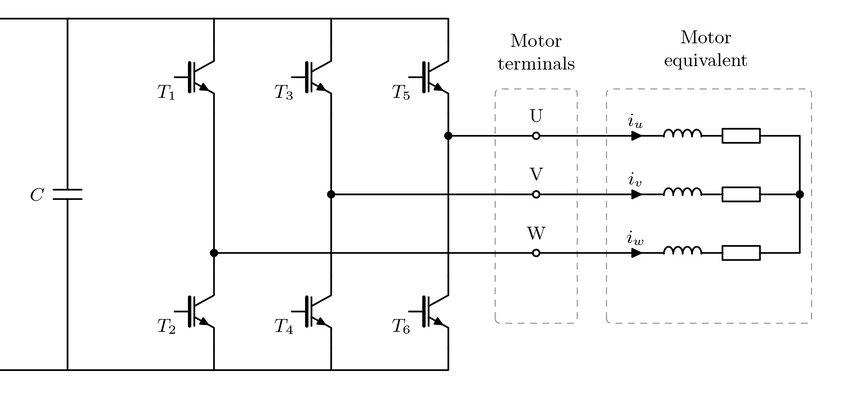
\includegraphics[width=0.9\textwidth]{Figs/2_inverter_structure.png}}
	\caption{Two-level inverter driving a 3-phase motor. Image source: \cite{InverterStruct}}
	\label{fig:0_inverter_structure}
\end{figure}
In theory, each of the six semiconductor switches can be controlled independently. However, during normal operation, the switches of a halfbridge are operated in a complementary manner. Turning on both switches simultaneously would short-circuit the DC link and cause a shoot-through event. To prevent this, a short dead time is typically introduced when changing between switching states, during which both switches of a half-bridge are turned off. During this interval, the stator current can continue to flow through the freewheeling diodes (or body diodes respectively).\\
Since the \acrshort{pmsm} considered here has no neutral connection, it will only react on the differential voltage signals with respect to the half bridge output nodes. Apart from the dead-time during interlocking, the state of the upper switch directly determines the state of the lower switch. With that, there are $2^3=8$ possible states in which the switches can be controlled. By defining $\bm{s}_{upper}^\T = [s_{a,u}\; s_{b,u}\; s_{c,u}]$ as the vector of the state of the upper switches, the set of all switching states can be written down:
\begin{equation}
	\mathcal{S}_{upper} = \left\{
	\begin{bmatrix}
		0 \\ 0\\ 0
	\end{bmatrix}, 
	\begin{bmatrix}
		0 \\ 0\\ 1
	\end{bmatrix},
	\begin{bmatrix}
		0 \\ 1\\ 0
	\end{bmatrix},
	\begin{bmatrix}
		0 \\ 1\\ 1
	\end{bmatrix},
	\begin{bmatrix}
		1 \\ 0\\ 0
	\end{bmatrix},
	\begin{bmatrix}
		1 \\ 0\\ 1
	\end{bmatrix},
	\begin{bmatrix}
		1 \\ 1\\ 0
	\end{bmatrix},
	\begin{bmatrix}
		1 \\ 1\\ 1
	\end{bmatrix}
	\right\}
    \label{equ:0_Supper}
\end{equation}
The first and last vector of $\mathcal{S}_{upper} $ result in identical voltages at all three half-bridge output nodes and therefore result in a zero stator voltage space vector. Thus, they are referred to as the zero voltage vectors. The remaining six active vectors can be used to direct the current flow through the machine.\\
By applying the Clarke transform to a vector of switching states, scaled by the DC-Link voltage of the inverter $U_{DC}$, the corresponding voltage space vectors can be determined.
\[
\begin{bmatrix}
	u_{\alpha} \\ u_{\beta}
\end{bmatrix} = 
U_{DC} \cdot \clarke \cdot
\begin{bmatrix}
	s_{a,u} \\ s_{b,u} \\ s_{c,u} 
\end{bmatrix}
\]
Applying this transformation to all eight switching states results in six equally spaced active voltage vectors and two zero voltage vectors located at the origin. The six active vectors form the well-known voltage hexagon of a \acrshort{2lvsi}, as depicted in Figure \ref{fig:0_SRF_hexagon}. This voltage hexagon defines the set of voltage space vectors that can be directly generated by the inverter.
\begin{figure}[H]
	\centering
	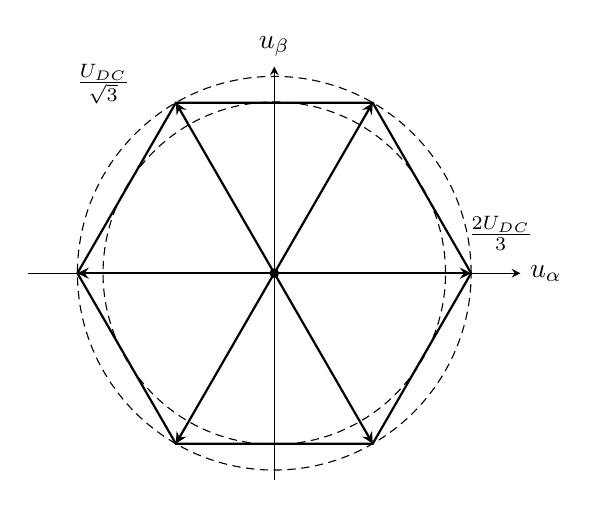
\begin{tikzpicture}[scale=2.5, >=stealth]

    \def\V{1}

    % axis
    \draw[->] (-1.25*\V,0) -- (1.25*\V,0)
        node[right] {$u_\alpha$};
    \draw[->] (0,-1.05*\V) -- (0,1.05*\V)
        node[above, at end] {$u_\beta$};

    % hexagon
    \draw[thick]
        (0:\V)
        -- (60:\V)
        -- (120:\V)
        -- (180:\V)
        -- (240:\V)
        -- (300:\V)
        -- cycle;

    % vectors
    \foreach \angle/\label in {
        0,
        60,
        120,
        180,
        240,
        300
    }{
        \draw[->, thick]
            (0,0) -- (\angle:\V)
            node[pos=1.15] {};
    }

    \fill (0,0) circle (0.7pt);
	\node (node1) at (-0.87,0.96) {$\frac{U_{DC}}{\sqrt{3}}$};
	\node (node2) at (1.15,0.2) {$\frac{2U_{DC}}{{3}}$};
  \draw[densely dashed] (0,0) circle (0.87cm);
\draw[densely dashed] (0,0) circle (1cm);
\end{tikzpicture}
	\caption{Voltage Hexagon in \acrshort{srf}}
	\label{fig:0_SRF_hexagon}
\end{figure}

\section{Model Predictive Control} \label{sec:0_mpc}
In Model Predictive Control (MPC), a model of the plant is used to predict its future behavior for a sequence of candidate control inputs. The control inputs are optimized with respect to a defined cost function while satisfying the relevant system constraints. \\
\begin{figure}[h]
    \centering
    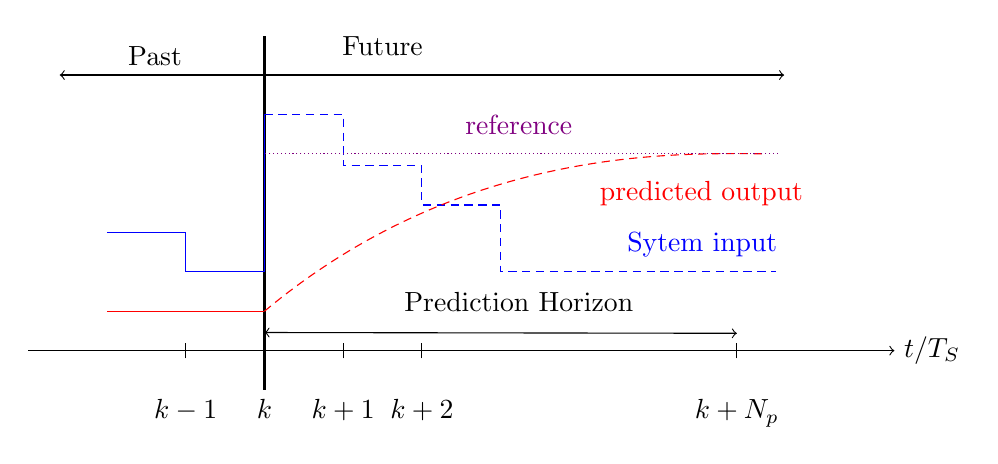
\begin{tikzpicture}
	% Timeline
	\draw[->] (-3, 0) -- (8, 0) node[right] {$t/T_S$};
	
	% Past/Future divider
	\draw[thick] (0, -0.5) -- (0, 4);
	\node[above] at (-1.39, 3.5) {Past};
	\node[above] at (1.5, 3.62) {Future};
	
	% Time axis labels
	\foreach \x/\label in {-1/k-1, 0/k, 1/k+1, 2/k+2, 6/k+N_p} {
		\draw (\x, -0.1) -- (\x, 0.1);
		\node[below] at (\x, -0.5) {$\label$};
	}

	% Arrows from past/future
	\draw[<-] (-2.6, 3.5) -- (0, 3.5);
	\draw[->] (0, 3.5) -- (6.6, 3.5);

  \draw[blue] (-2,1.5) -- (-1,1.5) -- (-1,1) -- (0,1) -- (0,3);

  \draw[densely dashed, blue] (0,3) -- (1,3) -- (1,2.35) -- (2,2.35) -- (2,1.85) -- (3,1.85) -- (3,1) -- (6.5,1);
  \draw[red] (0,0.5) -- (-2,0.5);
  \draw[densely dashed, red] (0,0.5) .. controls (2.56,2.64) and (5.34,2.5) .. (6.37,2.5);
  \draw[violet, densely dotted] (6.52,2.5) -- (0,2.5);
  \node[text=blue] at (5.56,1.34) {Sytem input};

  \node[text=red] at (5.55,2) {predicted output};

  \node[text=violet] at (3.23,2.87) {reference};

  \node[above] at (3.23, 0.37) {Prediction Horizon};
  \draw[<->] (0, 0.23) -- (6, 0.22);
\end{tikzpicture}
    \caption{Fundamentals of Model Predictive Control}
    \label{fig:0_mpc_scheme}
\end{figure}
For the prediction a mathematical model, such as a state space description, or a data-driven model is used. Using knowledge of plant states at the current sampling step $x(kT_S) = x[k]$ (with $k\in\mathbb{Z}$ and $T_S$ as the sampling time), an input-dependent prediction regarding the future behavior of the plant can be made. Since an MPC is typically implemented on a digital processor, a discrete number of future steps is used. This is typically referred to as the prediction horizon $N_P$. During this horizon, the effect of a discrete number of control inputs, also referred to as the control horizon $N_C$, with $N_C \le N_P$, on plant states and output is considered. As it will be explained in Section \ref{sec:2_op}, $N_C = N_P$ is used in this thesis. The plant inputs for the control horizon are chosen optimally with respect to a certain cost function $J$ and plant constraints. The cost function can be designed such that not only tracking errors are minimized but also other application-specific unwanted effects are punished. Due to the control law being formulated as an optimization problem, limits regarding plant inputs $u$ or states $x$ can be easily considered as constraints. By defining the set of valid plant states as $\mathcal{X}$ and valid inputs as $\mathcal{U}$, the optimization problem can be written down as the following
\begin{equation}
    \begin{split}
            \Bar{u}[k]^* &= \arg \min_{\Bar{u}[k]}\; J(\bar{u}[k])\\
	 \text{s.t.} \;x&\in \mathcal{X}\\
     u &\in \mathcal{U}
    \end{split}
    \label{equ:0_sample_op}
\end{equation}
In the Optimization Problem \eqref{equ:0_sample_op}, the prediction vector of input quantities used is defined as: 
\[
\Bar{u}[k] = \left[ u[k] \; u[k+1] \; \hdots \; u[k+N_C-1]   \right]^\T.
\]
and the optimal sequence $\Bar{u}[k]^* $ is the solution of that problem. Although $N_C$ control inputs are obtained by solving \eqref{equ:0_sample_op}, only the first control input is applied to the plant. At the next sampling instant, after obtaining the plant state by measurement or observation, the optimization problem is solved again, and the obtained first control input is applied. The method used, often known as the receding-horizon principle, is repeated at every sampling instant.\\
This framework allows for the usage of a compact control law, which is able to plan the future plant inputs while considering limits of complex Multiple-Input-Multiple-Output (MIMO) Systems. Another benefit of this control strategy is its flexibility for various extensions. As an example, for field oriented control, dead time compensation is a commonly used. With MPC this is easily achieved by defining the optimization problem for one step in time ahead (see Section \ref{sec:ext_deadt_comp}). \\
For field oriented current control of an \acrshort{pmsm}, the circular constraints of the stator currents $\boldsymbol{i}_{S} \in \mathcal{I}_S$ and the hexagonal input constraints regarding the stator voltage of the \acrshort{2lvsi} $\boldsymbol{u}_{S} \in \mathcal{U}_S$ must be obeyed. Since the stator voltage computed for the current step in time $\boldsymbol{u}_{S}^S[k]$ influences the stator current, which will be measured in the next step in time, the output constraints are formulated in terms of an estimation $\hat{\boldsymbol{i}}_{S}[k+1]$. For the sake of the argument in this example cost function an arbitrary vector norm of tracking error shall be minimized.
\[
\|\hat{\boldsymbol{i}}_{S}[k+1] -\boldsymbol{i}_{S,ref}[k+1]\| = \|\boldsymbol{e}_S[k+1]\| 
\]
Due to the receding horizon principle the trajectory of the tracking error is minimized, instead of the expected tracking error during the next period . To indicate such prediction vectors, a $\bar{\text{bar}}$ over the respective variable is used. 
\[
\Bar{\bm e}_S^\T[k+1] = \left[ \bm{e}_S^\T[k+1] \; \bm{e}_S^\T[k+2] \; \hdots \; \bm{e}_S^\T[k+N_P]   \right]
\]
Considering this, one could define an MPC control law as the following:

\begin{equation*}
	 \left( 
    \begin{split}
        \bar{\bm{u}}_S^*[k] = \arg \min_{\Bar{\bm{ u}_S}}\; &  \|  \Bar{\bm e}_S[k+1] \|\\
    	 \text{s.t.} \quad \bar{\boldsymbol{i}}_{S}[k+1] &\in \mathcal{I}_S \\
    	  \bar{\boldsymbol{u}}_{S}^S[k] &\in \mathcal{U}_{S} 
    \end{split}
    \right)\\
    \bm{u}_S[k] = [\I\; \bm{0} \; \hdots \; \bm{0}] \; \bar{\bm{u}}_S^*[k]
\end{equation*}
\subsection{Control Set Formulation}

The choice of the control set determines how the inverter voltage is represented and optimized in MPC. Depending on whether the control inputs are restricted to the discrete switching states or allowed to vary continuously within the feasible voltage region, MPC can be formulated as either Finite Control Set MPC (\acrshort{fcs}-MPC) or Continuous Control Set MPC (CCS-MPC).

\subsubsection{Finite Control Set}

In Finite Control Set MPC (\acrshort{fcs}-MPC), the possible control inputs are restricted to a finite set of predefined values. For the \acrshort{2lvsi} considered here, these inputs correspond directly to the eight possible switching states, defined in the set $\mathcal{S}_{upper}$ of Equation \eqref{equ:0_Supper}. The switching state is used directly as the control input of the inverter, eliminating the need for a separate modulation stage. The optimization problem is solved by evaluating the finite set of possible switching states and selecting the one that minimizes the defined cost function.\\ % vllt cite FCSCompWang as well
Due to the absence of a modulation stage, the FCS-MPC must adequately choose when to apply zero vectors. Considering this, the sampling time is usually chosen significantly smaller than for Continuous Control Set MPC.
As shown in \cite{NeunerMA} \cite{FCSCompBoek}, by choosing a sampling time $T_S$, which allows for solving the MPC optimization problem online, the resulting ripple on  the stator current is significant. Even though a variety of ripple mitigation strategies for FCS-MPC were introduced \cite{FCSCompLi}, a similar smoothness of output current and torque to \acrshort{pi}-FOC or \acrshort{ccs}-MPC cannot be achieved. Therefore this scheme is not considered in this thesis.

\subsubsection{Continuous Control Set}
In contrast to FCS-MPC, Continuous Control Set MPC (\acrshort{ccs}-MPC) formulation allow any voltage space vector, inscribed by the inverter hexagon to be used as a control input to the electric drive. For the \acrshort{2lvsi}, this region is given by the voltage hexagon shown in Figure \ref{fig:0_SRF_hexagon}.\\
To achieve the generation of control voltages which are not active voltage vectors or zero vectors, as defined in the set $\mathcal{S}_{upper}$ of Equation \eqref{equ:0_Supper} a modulation scheme is employed. To utilize all of the feasible region of the voltage hexagon, Space Vector Pulse Width Modulation (SVPWM) is typically used \cite{InverterStruct}. With \acrshort{ccs}-MPC, the stator current ripple depends on the switching frequency and the modulation scheme used. Compared to FCS-MPC with a similar sampling frequency, the current ripple is much lower in amplitude. Therefore, only CCS-MPC is considered in this thesis.


\subsection{Comparison to classical \acrshort{pi} field oriented control \label{sec:intro_comp_cs}}
Using classical field-oriented \acrshort{pi} \acrshort{foc}, the field-oriented control of a \acrshort{pmsm} can be achieved by splitting the voltage equation (as it will be derived in Section \ref{sec:model_pmsm}) up into two linear, decoupled subsystems and two coupling terms:
\begin{align*}
	\Dot{i_{Sd}}
	&=
	\underbrace{
		\frac{1}{L_d} u_{Sd} - \frac{R_S}{L_d} i_{Sd}
	}_{\Sigma_\mrm{d,decoupled}}
	+
	\underbrace{
		\frac{L_q}{L_d} \, i_{Sq}  \omega 
	}_{\Sigma_\mrm{d,coupled}}
	\\
	\Dot{i_{Sq}}
	&=
	\underbrace{
		\frac{1}{L_q} u_{Sq} - \frac{R_S}{L_q} i_{Sq}
	}_{\Sigma_\mrm{q,decoupled}}
	-
	\underbrace{
		\frac{L_d}{L_q} \,  i_{Sd} \omega
	}_{\Sigma_\mrm{q,coupled}}
	-
	\underbrace{
		\frac{1}{L_q} \, \psi_{PM} \omega 
	}_{\Sigma_\mrm{q,affine}}
\end{align*}
The linear systems $\Sigma_\mrm{d,decoupled}$ and $\Sigma_\mrm{q,decoupled}$ are controlled using two independent \acrshort{pi} controllers. The remaining coupling and back-\acrshort{emf} terms are compensated by a feed-forward system.\\
In contrast, CCS-MPC considers the complete coupled $dq$-model within its prediction model. The cross-coupling and back-\acrshort{emf} terms are therefore inherently considered when predicting the future current evolution, without requiring explicit decoupling through feed-forward compensation. Furthermore, the $d$- and $q$-axis voltage components are optimized simultaneously. \\
Another difference is the treatment of the inverter voltage constraint. In \acrshort{pi}-\acrshort{foc}, the voltage reference generated by the \acrshort{pi} controllers is typically limited subsequently by the modulation stage, requiring measures such as anti-windup to handle saturation. In \acrshort{ccs}-MPC, the voltage constraint can be included directly in the optimization problem.\\
To compensate for the switching and computation delay, Smith-Predictor based approaches are commonly used for field-oriented control of PMSMs. A few publications in this field resorted to predictive observer based approaches to cope with this problem \cite{XuchenPMSMiObs}. Both approaches require an additional system which compensates the delay. Since an MPC is build around a model-based prediction, including dead time compensation here, comes without additional computational effort. For details refer to Section \ref{sec:ext_deadt_comp}.